\section{最適フィードバック制御モデル}
ToDo: infiniteOFCと数式の統一を行う.

\subsection{最適フィードバック制御モデルの構造}
\textbf{最適フィードバック制御モデル (optimal feedback control; OFC)} の特徴として目標軌道を必要としないことが挙げられる.\textbf{Kalman フィルタ}による状態推定と\textbf{線形2次レギュレーター(LQR: linear-quadratic regurator)} により推定された状態に基づいて運動指令を生成という2つの流れが基本となる.
\subsubsection{系の状態変化}


\begin{align}
&\text {Dynamics} \quad \mathbf{x}_{t+1}=A \mathbf{x}_{t}+B \mathbf{u}_{t}+\boldsymbol{\xi}_{t}+\sum_{i=1}^{c} \varepsilon_{t}^{i} C_{i} \mathbf{u}_{t}\\
&\text {Feedback} \quad \mathbf{y}_{t}=H \mathbf{x}_{t}+\omega_{t}+\sum_{i=1}^{d} \epsilon_{t}^{i} D_{i} \mathbf{x}_{t}\\
&\text{Cost per step}\quad \mathbf{x}_{t}^\top Q_{t} \mathbf{x}_{t}+\mathbf{u}_{t}^\top R \mathbf{u}_{t}
\end{align}


\subsubsection{LQG}
加法ノイズしかない場合($C=D=0$),制御問題は\textbf{線形2次ガウシアン(LQG: linear-quadratic-Gaussian)制御}と呼ばれる.


\paragraph{運動制御 (Linear-Quadratic Regulator)}


\begin{align}
\mathbf{u}_{t}&=-L_{t} \widehat{\mathbf{x}}_{t}\\
L_{t}&=\left(R+B^{\top} S_{t+1} B\right)^{-1} B^{\top} S_{t+1} A\\
S_{t}&=Q_{t}+A^{\top} S_{t+1}\left(A-B L_{t}\right)\\
s_t &= \mathrm{tr}(S_{t+1}\Omega^\xi) + s_{t+1}; s_T=0
\end{align}


$\boldsymbol{S}_{T}=Q$

\paragraph{状態推定 (Kalman Filter)}


\begin{align}
\widehat{\mathbf{x}}_{t+1}&=A \widehat{\mathbf{x}}_{t}+B \mathbf{u}_{t}+K_{t}\left(\mathbf{y}_{t}-H \widehat{\mathbf{x}}_{t}\right)+\boldsymbol{\eta}_{t} \\ 
K_{t}&=A \Sigma_{t} H^{\top}\left(H \Sigma_{t} H^{\top}+\Omega^{\omega}\right)^{-1} \\ 
\Sigma_{t+1}&=\Omega^{\xi}+\left(A-K_{t} H\right) \Sigma_{t} A^{\top}
\end{align}


この場合に限り,運動制御と状態推定を独立させることができる.
\subsubsection{一般化LQG}
状態および制御依存ノイズがある場合,
\subsection{実装}
ライブラリの読み込みと関数の定義.
\lstinputlisting[language=julia]{./text/motor-learning/optimal-feedback-control/004.jl}
ToDo: struct 修正 (nが両方に入っている) 
\lstinputlisting[language=julia]{./text/motor-learning/optimal-feedback-control/006.jl}
Qの値は各時刻において一般座標 (位置,速度,加速度,躍度)のそれぞれを0にするコストに対する重みづけである.例えば,速度も0にすることを重視すれば2番目の係数を上げる.
$S$と$\Sigma$は各時点での値を一時的にしか必要としないので更新する.
\lstinputlisting[language=julia]{./text/motor-learning/optimal-feedback-control/009.jl}
\subsubsection{シミュレーション}
信号依存ノイズ Yが入っている場合はLQGとは異なってくる.


\begin{align}
&\mathbf{u}_{t}=-L_{t} \hat{\mathbf{x}}_{t} \\
&L_{t}=\left(B^\top S_{t+1}^{\mathbf{x}} B+R+\sum_{n} C_{n}^\top\left(S_{t+1}^{\mathbf{x}}+S_{t+1}^{\mathrm{e}}\right) C_{n}\right)^{-1} B^\top S_{t+1}^{\mathbf{x}} A \\
&S_{t}^{\mathbf{x}}=Q_{t}+A^\top S_{t+1}^{\mathbf{x}}\left(A-B L_{t}\right) ; \quad S_{T}^{\mathbf{x}}=Q_{T} \\
&S_{t}^{\mathrm{e}}=A^\top S_{t+1}^{\mathbf{x}} B L_t+\left(A-K_{t} H\right)^\top S_{t+1}^{\mathrm{e}}\left(A-K_{t} H\right) ; \quad S_{T}^{\mathrm{e}}=0\\
&s_{t}=\operatorname{tr}\left(S_{t+1}^{\mathrm{x}}\Omega^{\xi}+S_{t+1}^{\mathrm{e}}\left(\Omega^{\xi}+\Omega^{\eta}+K_{t} \Omega^{\omega} K_{t}^{\top}\right)\right)+s_{t+1} ; \quad s_{n}=0 .
\end{align}



\begin{align}
\hat{\mathbf{x}}_{t+1} &=A \hat{\mathbf{x}}_{t}+B \mathbf{u}_{t}+K_{t}\left(\mathbf{y}_{t}-H \hat{\mathbf{x}}_{t}\right) \\
K_{t} &=A \Sigma_{t}^{\mathrm{e}} H^\top\left(H \Sigma_{t}^{\mathrm{e}} H^\top+\Omega^{\omega}\right)^{-1} \\
\Sigma_{t+1}^{\mathrm{e}} &=\left(A-K_{t} H\right) \Sigma_{t}^{\mathrm{e}} A^\top+\sum_{n} C_{n} L_{t} \Sigma_{t}^{\hat{x}} L_{t}^\top C_{n}^\top ; \quad \Sigma_{1}^{\mathrm{e}}=\Sigma_{1} \\
\Sigma_{t+1}^{\hat{\mathbf{x}}} &=K_{t} H \Sigma_{t}^{\mathrm{e}} A^\top+\left(A-B L_{t}\right) \Sigma_{t}^{\hat{\mathbf{x}}}\left(A-B L_{t}\right)^\top ; \quad \Sigma_{1}^{\hat{\mathbf{x}}}=\hat{\mathbf{x}}_{1} \hat{\mathbf{x}}_{1}^\top
\end{align}
\lstinputlisting[language=julia]{./text/motor-learning/optimal-feedback-control/011.jl}
状態ノイズがある場合に関してはTodorovのMATLABコード \url{https://homes.cs.washington.edu/~todorov/software/gLQG.zip}を参照.

位置は目標位置を基準とする座標で表現し,位置が0になるように運動を行う.状態の中に標的位置を含めコストパラメータを修正することで初期位置を基準とする座標系での運動を記述できる.モデルに関してはTodorov2005を参照.
\lstinputlisting[language=julia]{./text/motor-learning/optimal-feedback-control/013.jl}
\lstinputlisting[language=julia]{./text/motor-learning/optimal-feedback-control/014.jl}
\lstinputlisting[language=julia]{./text/motor-learning/optimal-feedback-control/015.jl}
\lstinputlisting[language=julia]{./text/motor-learning/optimal-feedback-control/016.jl}
\begin{figure}[ht]
	\centering
	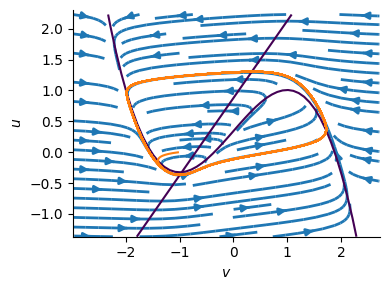
\includegraphics[scale=0.8, max width=\linewidth]{./fig/neuron-model/fhn/cell016.png}
	\caption{cell016.png}
	\label{cell016.png}
\end{figure}
\lstinputlisting[language=julia]{./text/motor-learning/optimal-feedback-control/017.jl}
\begin{figure}[ht]
	\centering
	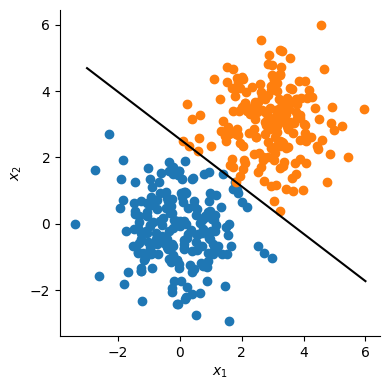
\includegraphics[scale=0.8, max width=\linewidth]{./fig/local-learning-rule/logistic-regression-perceptron/cell017.png}
	\caption{cell017.png}
	\label{cell017.png}
\end{figure}
